\section{Entscheidungen unter Risiko}
\label{Risiko}

Bisher haben wir nur über Entscheidungen unter Unwissenheit gesprochen. Damit
sind solche Entscheidungen gemeint, bei denen wir die Menge der möglichen
Ereignisse, die -- unabhängig von unserer Wahl -- auf das Ergebnis Einfluss
nehmen können, genau kennen, bei denen wir aber nicht wissen, mit welcher
Wahrscheinlichkeit jedes der Ereignisse eintreten wird. In diesem Kapitel
werden wir die Techniken des Umgangs mit "`Entscheidungen unter Risiko"' kennen
lernen, wobei mit Entscheidungen unter Risiko genau solche Entscheidungen
gemeint sind, bei denen wir die Wahrscheinlichkeiten für das Eintreten der
Ereignisse (oder der Gegebenheit bestimmter Zustände kennen). Bei
Entscheidungen unter Risiko verfügen wir also über mehr Informationen als bei
Entscheidungen unter Unwissenheit. In diesem Sinne ist Risiko (so wir der
Begriff innerhalb der Entscheidungstheorie verstanden wird) günstiger als
Unwissenheit. 

Da wir bei Entscheidungen unter Risiko Wahrscheinlichkeiten voraussetzen, müsste,
wollte man nach der logischen Reihenfolge vorgehen, eigentlich zuvor der
mathematische Wahrscheinlichkeitsbegriff eingeführt werden. Weil die
Wahrscheinlichkeitstheorie aber eine komplizierte Sache ist, wird die
Wahrscheinlichkeitstheorie aus didaktischen Gründen erst später besprochen. Bis
dahin genügt es, über Wahrscheinlichkeiten lediglich das folgende zu wissen:

\begin{enumerate}
  \item Jede Wahrscheinlichkeit $p$ ist eine Zahl von $0$ bis $1$, also $ 0
  \leq p \leq 1$. Eine Wahrscheinlichkeit von $0$ bedeutet, dass ein Ereignis
  "`praktisch unmöglich"' ist, eine Wahrscheinlichkeit von $1$, dass es
  "`praktisch sicher"' ist.
  \item Die Wahrscheinlichkeiten von Ereignissen, die sich ausschließen kann
  man addieren und man erhält dabei die Wahrscheinlichkeit, dass das eine {\em
  oder} das andere Ereignis eintritt. Also, seien $E$ und $F$ zwei Ereignisse,
  die sich wechselseitig ausschließen, dann gilt $P(E) + P(F) = P(E \vee F)$.
  \item Bei einer Menge von einander sich wechselseitig ausschließenden ({\em
  paarweise disjunkten}) Ereignissen, von denen aber irgendeins auf jeden Fall
  eintritt ({\em erschöpfende Ereignismenge}) addieren sich die
  Wahrscheinlichkeiten zu $1$ auf. 
\end{enumerate}


\subsection{Die Berechnung des Erwartungsnutzens}
\label{Erwartungsnutzenhypothese}
Um unter Risiko eine begründete Entscheidung treffen zu können, müssen wir den
Nutzen unsicherer Ereignisse in irgendeiner Weise bewerten, so dass die
Unsicherheit bzw. das Risiko bei der Bewertung mit einbezogen wird. 
Dieser Nutzenwert, in den die Unsicherheit schon mit eingerechnet ist, wird der
{\em Erwartungsnutzen} genannt. Da im Erwartungsnutzen der Nutzen eines
Ereignisses mit dem Wert des Ereignisses, wenn es eintritt, verrechnet wird,
setzt die Bestimmung des Erwartungsnutzen immer ein kardinales Nutzenkonzept
voraus.

Das zentrale Gesetz des Erwartungsnutzens ist die sogenannte
Erwartungsnutzenhypothese. Sie besagt, dass der Erwartungsnutzen eines
unsicheren Ereignisses gleich dem erwarteten Nutzen multipliziert mit der
Wahrscheinlichkeit des Eintretens des Ereignisses ist. Unter dem
"`Erwartungsnutzen"' ist dabei der Nutzen des noch {\em unsicheren} Ereignisses
zu verstehen. Während mit dem "`erwarteten Nutzen"' der Nutzen des Ereignisses
(für einen bestimmten Akteur) gemeint ist, wenn dass Ereignis eingetreten ist.
"`Erwartungsnutzen"' und "`erwarteter Nutzen"' dürfen also nicht verwechselt
werden! Der Zusammenhang kann also mathematisch folgendermaßen formuliert werden:

\marginline{Erwartungs\-nutzen}
\begin{equation*}
    EU = p \cdot U \label{EN1}
\end{equation*}

\begin{center}
\begin{tabular}{ll}
EU & Erwartungsnutzen eines bestimmten Ereignisses \\
 p & Wahrscheinlichkeit des Eintretens dieses Ereignisses \\
 U & Nutzen des eingetretenen Ereignisses ("`erwarteter Nutzen"')\\
\end{tabular}
\end{center}
Wird der Zusammenhang so wie in der Gleichung oben ausgedrückt, dann wird
dabei stillschweigend vorausgesetzt, dass der erwartete Nutzen, wenn das
Ereignis nicht eintritt, Null beträgt. In etwas präziserer und allgemeinerer
Form müsste man den Zusammenhang so darstellen: 

Sei $e_1,\ldots ,e_n$ eine
{\em Partition} von Ereignissen, d.h. eine Menge von Ereignissen, die sich
wechselseitig ausschließen, von denen eins aber eintreten muss. Seien weiterhin
die Wahrscheinlichkeiten, mit denen diese Ereignisse eintreten können:
$p_1,\ldots ,p_n$ und ihre erwarteten Nutzenwerte $U_1,\ldots ,U_n$. Dann
berechnet sich der Erwartungsnutzen nach:\label{Erwartungsnutzen}
\begin{equation*}
    EU = p_1 \cdot U_1 + p_2 \cdot U_2 + \ldots + p_n \cdot U_n
\end{equation*}

 Die Berechnung des Erwartungsnutzens hat aber offensichtlich nur
dann Sinn, wenn wir eine {\em kardinale Nutzenfunktion} (siehe Kapitel
\ref{KardinalerNutzen}) voraussetzen dürfen, da der so berechnete
Erwartungsnutzuen nicht bei jeder positiven Transformation der gewählten
Nutzenfunktion derselbe bleibt. Sie ist aber insbesondere dann unproblematisch,
wenn es sich bei dem Nutzen um Geldwerte handelt. Dass unter der Voraussetzung
kardinaler Nutzenwerte die Verwendung des Erwartungsnutzens zur Bewertung
unterschiedlicher Handlungsalternativen unbedenklich ist, ergibt sich daraus,
dass der Erwartungsnutzen von positiv linear transformierten Nutzenwerten gleich
dem positiv linear transformierten Erwartungsnutzen der Nutzenwerte ist.
Mathematisch gesprochen: Seien $u$ und $v$ zwei äquivalente kardinale
Nutzenskalen, d.h. es gelte: $v = au + b$ mit $a > 0$. Dann gilt:
\begin{eqnarray*}
EV & = & p_1 \cdot V_1 + \ldots + p_n \cdot V_n \nonumber \\
{ }  & = & p_1 \cdot (aU_1 + b) + \ldots + p_n \cdot (aU_n + b) \nonumber \\
{ }  & = & ap_1 \cdot U_1 + \ldots + ap_n \cdot U_n + \sum_{i=1}^n p_ib
\nonumber \\ 
{ }  & = & a(p_1 \cdot U_1 + \ldots + p_n \cdot U_n) + b \nonumber
\\ & = & aEU + b 
\end{eqnarray*}
\begin{quote}{\em Hinweis}: Da $p_1+\ldots+p_n=1$ (es handelt sich um eine
Partition von Ereignissen, d.h. die Ereignisse schließen sich wechselseitig
aus und ein Ereignis tritt auf jeden Fall ein), durften wir im
vorletzten Schritt $\sum_{i=1}^n p_ib = b\cdot \sum_{i=1}^n p_i = b \cdot 1 = b$
verwenden.\end{quote}

Bewertet man den Wert unterschiedlicher Handlungsalternativen
einer Entscheidung unter Risiko (d.i. einer Entscheidung, bei der die
Eintrittswahrscheinlichkeiten der möglichen Zufallsereignisse bekannt sind) mit
Hilfe des Erwartungsnutzens, so ist damit sichergestellt, dass die Rangfolge der
Alternativen dieselbe bleibt, wenn wir unsere Nutzenfunktion durch eine
äquivalente kardinale Nutzenfunktion ersetzen. 

% Denn sei $EU_A$ der einer
% Handlungsalternative $A$ zugeordnete Erwartungsnutzen und $EU_B$ der einer
% Handlungsalternative $B$ zugeordnete Erwartungsnutzen und gelte:
% \[ EV_A = aEU_A + b \]
% \[ EV_B = aEU_B + b \]
% Dann folgt aus aus $EU_A > EU_B$ für positive $a$ offensichtlich, dass auch
% $EV_A > EU_B$ und aus $EU_A = EU_B$, dass $EV_A = EU_B$  

Aus dem Erwartungsnutzen ergibt sich eine sehr einfache Entscheidungsregel für
Entscheidungen unter Risiko, sofern die erwarteten Werte mindestens auf einer
kardinalen Nutzenskala eingetragen werden können, nämlich die Regel:
 
\begin{quote}\label{Erwartungsnutzenregel}
{\em Entscheidungsregel für Entscheidungen unter Risiko}: Wähle
\marginline{Entscheidungs\-regel unter Risiko}
die\-jenige Entscheidung, bei der der Erwartungsnutzen % $EU = \sum_i p_iU_i$ 
am größten ist.
\end{quote}

Dass diese Regel bei Entscheidungen unter Risiko tatsächlich die beste ist,
werden wir gleich noch ausführlicher begründen. Wenn sie aber die beste ist, dann
ergibt sich für Unterscheidungen unter Risiko, dass wir nicht -- wie bei
Entscheidungen unter Unwissenheit -- mit dem Problem zu kämpfen haben, dass es
eine Reihe unterschiedlicher Entscheidungsregeln gibt, die alle sinnvoll
begründet werden können, die aber unter Umständen unterschiedliche Ergebnisse
liefern. (Inwiefern dies ein ernstzunehmendes Problem ist, sei dahin gestellt.
Man könnte es auch so interpretieren, dass es bei Entscheidungen unter
Unwissenheit eben keine generell beste Entscheidungsregel gibt, sondern nur
situationsspezifisch mehr oder weniger angemessene Entscheidungsregeln -- wobei
einmal angenommen sei, dass die Auswahl der richtigen Entscheidungsregel unter
Berücksichtigung der näheren situtationsspezifischen Bedingungen und Umstände
leichter fällt.)

\subsubsection{Beispiele}

Wie kann man mit Hilfe dieser Entscheidungsregel Entscheidungen unter Risiko
treffen? Dazu ein Beispiel.\label{RisikoBeispiel1} Eine Computerfirma hat
erfahren, dass die Konkurrenz dabei ist, eine neue Art von sehr preiswerten 
Kleinstlaptops zu
entwickeln. Sie steht nun vor der Wahl, ob sie ebenfalls in die Entwicklung
derartiger Laptops investieren soll. Es steht nicht fest, ob diese Art Laptops
vom Markt akzeptiert wird. Auch hängt der zu erwartende Gewinn davon ab, ob es
der Konkurrenz gelingt, noch in diesem Jahr ihr Produkt auf den Markt zu
werfen, in welchem Fall man die Eigenentwicklung zu einem deutlich niedrigeren
Preis mit entsprechend reduzierten Gewinnerwartungen anbieten müsste.
Andererseits ist zu erwarten, dass eine erfolgreiche Konkurrenz durch
Kleinstlaptops die Firma auch Marktanteile in ihren Kernbereichen kosten könnte.
Daraus ergibt sich folgendes Entscheidungsproblem:
\begin{center}
\marginline{Handlungs\-unab\-hängige Wahrscheinlichkeiten}
\begin{tabular}{c|r|r|r|r}
\multicolumn{1}{c}{}  & \multicolumn{1}{c}{$S_1$ ($p=0.3$)}  &
\multicolumn{1}{c}{$S_2$ ($p=0.2$)} & \multicolumn{1}{c}{$S_3$ ($p=0.5$)} & 
\multicolumn{1}{c}{} \\
\cline{2-4} $A_1$ & -100.000 € & -50.000 & € 60.000 & $EU = -10.000$ €\\ 
\cline{2-4} $A_2$ & 0 €        & -80.000 & € 0      & $EU = -16.000$ €\\ 
\cline{2-4}
\end{tabular}
\begin{tabular}{llp{11.5cm}}
& & \\
$A_1$: & & Investiere in die rasche Entwicklung eines Kleinstlaptops.\\
$A_2$: & & Investiere nicht in die Entwicklung eines Kleinstlaptops.\\
& &\\
$S_1$: & & Kleinstlaptops bleiben auf dem Markt erfolglos.\\
$S_2$: & & Kleinstlaptops sind erfolgreich, aber die Konkurrenz
                   ist ebenfalls frühzeitig auf dem Markt präsent.\\
$S_3$: & & Kleinstlaptops sind erfolgreich, aber die Entwicklung 
                   der Kon\-kurrenz verzögert sich. \\
\end{tabular}
\end{center}
Der Erwartungsnutzen der jeweiligen Handlungen wurde dabei folgendermaßen
errechnet:
\begin{eqnarray*}
EU_{A1} & = & -100.000 \cdot 0.3 - 50.000 \cdot 0.2 + 60.000 \cdot 0.5 =
-10.000 \\ 
EU_{A2} & = & 0 \cdot 0.3 - 80.000 \cdot 0.2 + 0 \cdot 0.5 = -16.000
\\
\end{eqnarray*}

Wie man an dem berechneten Erwartungsnutzen sieht, lohnt sich 
die Investition in die Entwicklung eines Kleinstlaptops, obwohl auch in diesem
Fall ein Verlust zu erwarten ist. \label{BeispielKausaleEntscheidung} Es kann
Entscheidungsprobleme geben, bei denen nicht nur die Nutzenwerte, 
sondern auch die Wahrscheinlichkeit, mit der
ein Ereignis eintritt, davon abhängt, welche Handlungsalternative man wählt. In
diesem Fall müssen die Wahrscheinlichkeiten für die möglichen Ereignisse in
jeder Zeile separat mit angegeben werden. Für die Berechnung des
Erwartungsnutzens müssen dann natürlich die Wahrscheinlichkeiten der
entsprechenden Zeile herangezogen werden. 
Ein Beispiel: Ein großes Softwareunternehmen
möchte im Laufe der nächsten Monate ein kleines Softwareunternehmen aufkaufen.
Es besteht die Möglichkeit, dass der Aktienkurs des Kleinunternehmens in den
folgenden Monaten sinkt, steigt oder gleich bleibt, worüber die Experten des
Großunternehmens relativ zuverlässige Schätzungen abgeben können. 
Das Großunternehmen kann seine
Kaufabsicht vorher ankündigen oder auch nicht. Kündigt es die Kaufabsicht
vorher an, so erhöht das die Wahrscheinlichkeit, dass der Aktienkurs und damit
der Preis des Kleinunternehmens steigt. Zugleich führt dies aber dazu, dass das
Kleinunternehmen, das bisher ein direkter Konkurrent des Großunternehmens ist,
bis zum Verkauf kaum noch Lizenzen absetzen kann, woraus sich in diesem Fall
ein fixer Gewinn für das Großunternehmen ergibt. Das Entscheidungsproblem sieht
als Tabelle folgendermaßen aus (Die eingetragenen Werte repräsentieren dabei
die Gesamtkosten, die sich aus dem zu erwartenden Kaufpreis minus dem fixen
Gewinn aus zusätzlichen Lizenzverkäufen nach Wegfall einer effektiven
Konkurrenz infolge der Ankündigung ergeben):
\begin{center}
\marginline{Handlungs\-abhängige Wahrscheinlichkeiten}
\begin{tabular}{c|l|l|l|l}
\multicolumn{1}{c}{}  & \multicolumn{1}{c}{Kurs steigt}  &
\multicolumn{1}{c}{Kurs fällt} & \multicolumn{1}{c}{bleibt gleich} &
\multicolumn{1}{c}{EU}\\
\cline{2-4} $A_1$: & 5 Mio € {\tiny(p=0.1)}                        
                   & 2 Mio € {\tiny(p=0.6)}
                   & 4 Mio € {\tiny(p=0.3)}
                   & 2.9 Mio €\\ 
                  
\cline{2-4} $A_2$: & 4.5 Mio € {\tiny(p=0.7)}
                   & 1.5 Mio € {\tiny(p=0.1)}
                   & 3.5 Mio € {\tiny(p=0.2)}
                   & 4 Mio €\\
\cline{2-4}
\end{tabular}
\begin{small}
\begin{tabular}{llp{11.5cm}}
& & \\
$A_1$ & & Kündige die Akquise {\em nicht} vorher an.\\
$A_2$ & & Kündige die Akquise vorher an.\\
\end{tabular}
\end{small}
\end{center}
Dies mal sieht die Berechnung des Erwartungsnutzens folgendermaßen aus:
\begin{eqnarray*}
EU_{A1} & = & 5.000.000 \cdot 0.1 + 2.000.000 \cdot 0.6 + 4.000.000 \cdot 0.3 =
2.900.000 \\ 
EU_{A2} & = & 4.500.000 \cdot 0.7 + 1.500.000 \cdot 0.1 + 3.500.000 \cdot 0.2 =
4.000.000 \\
\end{eqnarray*}
Da es sich bei den eingetragenen Werten um Kosten handelt, sollte das
Unternehmen tunlichst vermeiden, die Akquiseabsichten vorher anzukündigen.

Schließlich wollen wir noch an einem Beispiel betrachten, wie man den
Erwartungsnutzen einsetzt, um Entscheidungsbäume aufzulösen.
 Eine Ölfirma erwägt an einer
bestimmten Stelle in der Nordsee nach Öl zu bohren. Es ist nicht absolut sicher, 
ob sich an dem entsprechenden Ort
tatsächlich Öl befindet. Um dies mit Sicherheit festzustellen, kann die Firma
eine Probebohrung durchführen lassen. Der Bau einer Bohrinsel
kostet € 1.000.000. Liefert die Bohrinsel tatsächlich Öl, so erwirtschaftet die
Ölfirma mit dem geförderten Öl € 10.000.000. Die Durchführung einer
Expertise mit Hilfe einer Probebohrung kostet € 250.000. Wir gehen der
Einfachheit halber davon aus, dass die Probebohrung absolut zuverlässig darüber 
Auskunft gibt, ob Öl vorhanden
ist. Weiterhin sei angenommen, dass die Wahrscheinlichkeit, dass Öl vorhanden
ist 40\% beträgt. Um einen entsprechenden Entscheidungsbaum für Entscheidungen
unter Risiko zu zeichnen, werden die Wahrscheinlichkeiten für
Zufallsereignisse jeweils auf den entsprechenden Zweigen nach dem
Ereignisknoten eingetragen. Der Entscheidungsbaum sieht dann folgendermaßen aus:
\begin{center}
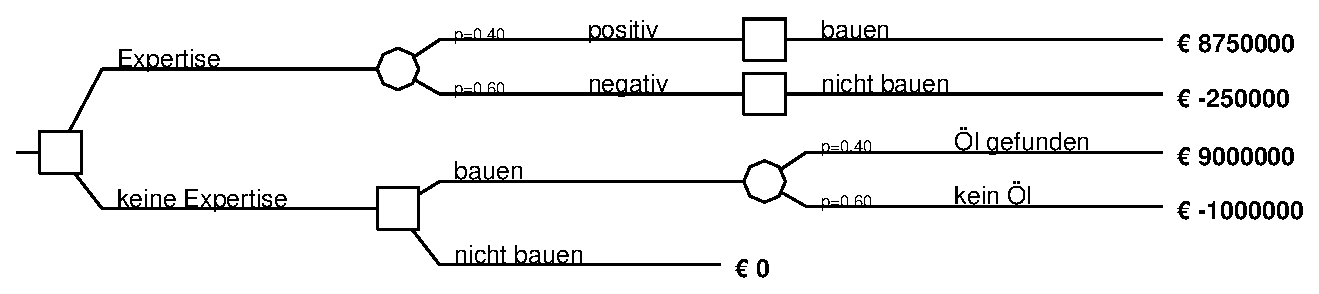
\includegraphics[width=12cm]{Grafiken/Beispiel6_3A.eps}
\end{center}
Wie kann man nun die Frage klären, ob es sich lohnt eine Expertise durchführen
zu lassen oder nicht? Dazu muss man den Entscheidungsbaum von rechts nach links
schrittweise nach folgenden Regeln auflösen:
\begin{enumerate}
  \item Ersetze jeden {\em Ereignis}knoten (der letzten Ebene) durch den
  Erwartungsnutzen des entsprechenden Ereignisses.\marginline{Regeln zur
  Auflösung von Entscheidungsbäumen}
  \item Ersetze jeden {\em Entscheidungs}knoten (der letzten Ebene) durch den
  (Erwartungs-)Wert der besseren Alternative.
  \item Führe das Verfahren fort bis die gesuchte (Teil-)Entscheidung erreicht
  ist.
\end{enumerate} 
In unserem Fall ist die gesuchte Entscheidung die Anfangsentscheidung, ob eine
Expertise durchgeführt werden soll. Wenn man den Baum nach dem entsprechenden
Verfahren reduziert, dann sieht der Entscheidungsbaum nach dem ersten Schritt
so aus:
\begin{center}
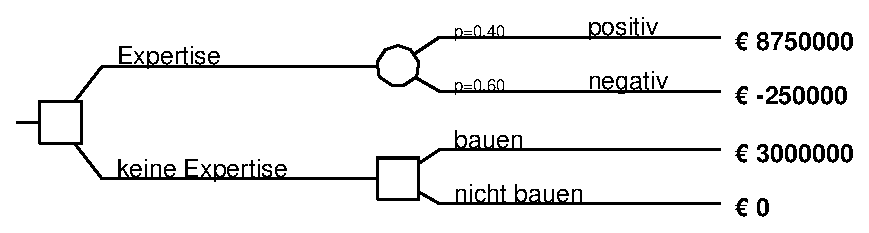
\includegraphics[width=10cm]{Grafiken/Beispiel6_3B.eps}
\end{center}
Der Erwartungswert, den man erhält, wenn man die Bohrinsel baut, ohne eine
Expertise durchzuführen beträgt € 3.000.000 (= € $0.4 \cdot 9.000.000 - 0.6
\cdot 1.000.000$). Dieser Erwartungswert wurde an die Stelle des entsprechenden
Ereignisknotens gesetzt. Da im anderen Fall die Entscheidung zum Bau
mit dem Ausgang der Expertise schon feststeht, wurden hier einfach die
entsprechenden Werte übertragen. Da der Bau der Ölplattform auch ohne vorherige
Probebohrung einen höheren Erwartungswert als 0 € liefert, muss für den letzten
Schritt nur noch der Erwartungsnutzen berechnet werden, der sich ergibt, wenn
man sich dazu entscheidet, die Expertise durchzuführen. Der nochmals reduzierte
Entscheidungsbaum sieht dann so aus:
\begin{center}

\includegraphics[width=6cm]{Grafiken/Beispiel6_3C.eps}
\end{center}
Es ist nun unmittelbar ersichtlich, dass es besser ist, vorher eine Expertise
in Auftrag zu geben, da der daraus resultierende Erwartungswert der größere
ist. 

Bei all diesen Beispielen haben wir übrigens eine Frage offen gelassen, die in
der praktischen Anwednung des Erwartungsnutzens von entscheidender Bedeutung
sein kann, nämlich die Frage, woher wir die Wahrscheinlichkeiten kennen, und ob
wir sicher sein können, dass die Wahrscheinlichkeiten für das Eintreten der
Ereignisse stimmen, wenn wir schon nicht sicher sein können, welches Ereignis
eintritt. Im Einzelfall dürfte dies von der Verfügbarkeit und Zuverlässigkeit
wissenschaftlicher Theorien abhängen, die diese Wahrscheinlichkeiten für den
entsprechenden Anwendungsbereich bestimmen.

\subsection{Die Rechtfertigung des Erwartungsnutzens}
\label{RechtfertigungErwartungsnutzen}
Soeben wurde gezeigt, wie man mit Hilfe des Erwartungsnutzens auf einfache
Weise Entscheidungsprobleme lösen kann. Zugleich wurde behauptet, dass der
Ewartungsnutzen bei Entscheidungen unter Risiko im Grunde die einzig sinnvolle
Entscheidungsregel darstellt. Aber warum ist das so? 

Eine Antwort auf diese Frage ist die, dass man, wenn man bei Entscheidungen unter
Risiko den Erwartungsnutzen zu Grunde legt, {\em auf lange Sicht} den größten
\marginline{Erwartungs\-nutzen ist auf lange Sicht gewinnmaximierend}
Gewinn erzielen kann.\footnote{Auch hier gibt es natürlich diskussionsbedürftige
Grenz- und Zweifelsfälle, wie z.B. \cite{okasha:2007} vor Augen führt.} Um sich
das klar zu machen nehme man eine Entscheidungssituation an, in der man entweder
einen festen Geldbetrag erhalten kann, oder mit einer bestimmten
Wahrscheinlichkeit einen höheren Geldbetrag. Z.B. könnte eine Person vor der
Entscheidung stehen, ob sie mit 5 € Einsatz an einer Lotterie teilnehmen will,
bei der sie mit 3\% Wahrscheinlichkeit 100 € gewinnen kann, oder ob sie das Geld
lieber behält. Behält sie das Geld, so entspricht das einem sicheren Gewinn von
5€. Wird diese Entscheidungssituation viele Male wiederholt, dann besagt das
Gesetz der Großen Zahlen aus der Statistik, dass der Grenzwert der Häufigkeit, mit der
ein bestimmtes Ereignis eintritt (in diesem Fall der Gewinn der Lotterie) mit der
Wahrscheinlichkeit 1 (also "`praktisch immer"') der Wahrscheinlichkeit des
Ereignisses entspricht. Handelt es sich bei der Wahrscheinlichkeit des Ereignisses um eine empirisch-statistische
Wahrscheinlichkeit und legt man die Häufigkeitstheorie der Wahrscheinlichkeit zu
Grunde (siehe Kapitel \ref{Haeufigkeitstheorie}), so gilt sogar, dass der
Grenzwert der Häufigkeit mit Sicherheit der Wahrscheinlichkeit des Ereignisses
entspricht.\footnote{"`Mit Sicherheit"' und "`mit Wahrscheinlichkeit 1"' ist
nicht, wie man denken könnte, ein- und dasselbe. Beispiel: Die Wahrscheinlichkeit
dafür, dass eine unendliche Folge von Münzwürfen nicht jedes mal Kopf liefert
befträgt 1. Trotzdem ist diese Ereignis nicht absolut sicher, denn das inverse
Ereignis, dass eine unendliche Folge von Münzwürden jedesmal Kopf liefert, ist
immerhin möglich.} Einfach ausgedrückt bedeutet dies: Wir können bei
hinreichend häufiger Wiederholung getrost davon ausgehen, dass das Ereignis genau so oft
eintritt, wie es seiner Wahrscheinlichkeit entspricht. In diesem Fall hieße das,
dass drei Prozent der Lotterien gewonnen werden. Bei einem Gewinn von 100 € wird
man auf lange Sicht 3 € pro Lotterie eingenommen haben, was genau dem
Erwartungswert der Lotterie $EU=0.03 \cdot 100$ € entspricht. Damit ist die
Lotterie aber deutlich weniger wert als der Einsatz von 5 €. Zumindest auf lange
Sicht sollte man immer den Erwartungswert (gleich Wahrscheinlichkeit mal
erwarteter Wert) für die Bewertung von Zufallsereignissen zu Grunde legen. Oder,
anders gesagt, man soll Zufallsereignisse weder zu optimistisch noch zu
pessimistisch bewerten, sondern genau entsprechend ihrer Wahrscheinlichkeit.

Dieselbe Argumentation lässt sich auch auf beliebige kardinale Nutzenwerte
übertragen, sofern man die Geldwerte durch Nutzenwerte ersetzt und statt des
Erwartungs{\em wertes} mit dem Erwartungs{\em nutzen} rechnet.

Die Argumentation weist zwei Schwierigkeiten auf: \marginline{Mögliche Einwände}
Erstens gilt sie nur auf lange Sicht, und es stellt sich zumindest die Frage, ob
man das, was auf lange Sicht gilt, auch auf einzelne Zufallsereignisse, die sich
in derselben Form nicht wiederholen, übertragen darf. Zweitens lässt sie sich --
wie schon erwähnt -- nur bei kardinalen Nutzenwerten anwenden, da wir sonst den
Erwartungsnutzen nicht einmal bestimmen können. Für beide Probleme versucht die
Neumann-Morgensternsche Nutzentheorie eine Lösung anzubieten. Für das erste
Problem, indem sie zeigt, dass der Erwartungsnutzen aus bestimmten
Konsistenzbedingungen hervorgeht, die verletzt werden, wenn man ihn nicht richtig
als das Produkt aus erwartetem Nutzen und Wahrscheinlichkeit berechnet -- ähnlich
wie subjektive Wahrscheinlichkeiten inkonsistent werden, sobald man die Axiome
der Wahrscheinlichkeitsrechnung verletzt (siehe
\ref{SubjektiveWahrscheinlichkeiten}). Für das zweite Problem, indem sie aus
einer beliebigen Präferenzrelation -- die aber reich genug sein muss, um auch
gedachte Güter von der Form sogenannter "`Lotterien"' zu enthalten! -- durch
trickreiche Vergleiche eine kardinale Nutzenfunktion konstruiert. Diese Theorie
werden wir später im Semester noch ausführlich besprechen (Kapitel
\ref{NeumannMorgenstern}).

\subsection{Kausale Entscheidungstheorie}

Bei einem der eben besprochenen Beispiele (Seite
\pageref{BeispielKausaleEntscheidung}) hingen die Wahrscheinlichkeiten, mit denen
Ereignisse eintreten, von den gewählten Handlungen ab.\footnote{Das
Hellseherparadox (Kapitel \ref{Hellseherparadox}) liefert ein weiteres, wenn
auch, da es echte hellseherische Fähigkeiten voraussetzt, sehr konstruiertes
Beispiel dafür.} Grundsätzlich werden solche Entscheidungsprobleme so gelöst,
dass wir die (handlungsabhängige) Wahrscheinlichkeit jedes möglichen Ergebnisses
in der entsprechenden Tabellenzelle vermerken und beim Ausrechnen des
Erwartungsnutzens für jede Handlung die in der entsprechenden Zeile vermerkten
Wahrscheinlichkeiten berücksichtigen.

Wir können nun noch einen Schritt weitergehen und uns fragen, wie vorzugehen
ist, wenn die Wahrscheinlichkeiten des Eintretens von Ereignissen nicht nur von den
Handlungen sondern wiederum von anderen Ereignissen und Zuständen abhängig sind.
Dazu ein Beispiel (frei nach Resnik \cite[S. 114]{resnik:1987}): Eine Ärztin
steht vor der Frage, ob sie die Infektion eines Patienten mit einem
Desinfektionsmittel oder mit einem Antibiotikum behandeln soll. Das
Antibiotikum schlägt bei 80\% der Patienten gut an, in welchem Fall die
Heilungschance bei 70\% liegt. Bei den restlichen Patienten liegt die
Heilungschance mit demselben Mittel jedoch nur bei 40\%. Das
Desinfektionsmittel hat dagegen bei allen Patienten eine Heilungschance von 50\%
Da beide Mittel, wie wir einmal annehmen wollen miteinander unverträglich sind,
besteht nur die Wahl entweder das Antibiotikum zu versuchen oder das
Desinfektionsmittel.

Um das Problem in einer Entscheidungstabelle darzustellen, kann man die
Ereignisse in zwei Gruppen unterteilen: Unabhängige und Abhängige Ereignisse. In
diesem Fall ist das unabhängige Ereignis, dasjenige, ob das Antibiotikum bei dem
Patienten anschlägt oder nicht. Das kausal davon abhängige Ereignis ist die
Heilung (oder Nicht-Heilung) des Patienten. Dabei müssen für jedes unabhängige
Ereignis alle abhängigen Ereignisse gesondert eingetragen werden. Wichtig ist,
dass man innerhalb der Tabelle die entsprechenden bedingten Wahrscheinlichkeiten
einträgt. Daraus ergibt sich folgende Entscheidungstabelle:
\begin{center}
\begin{footnotesize}
\begin{tabular}{c|c|c|c|c|}
\multicolumn{1}{c}{} & \multicolumn{2}{c}{A. schlägt an (80\%)} 
                     & \multicolumn{2}{c}{schlägt nicht an (20\%)} \\
\multicolumn{1}{c}{} & \multicolumn{1}{c}{Heilung (70\%)}
                     & \multicolumn{1}{c}{$\neg$Heilung (30\%)}
                     & \multicolumn{1}{c}{Heilung (40\%)}
                     & \multicolumn{1}{c}{$\neg$Heilung (60\%)}
                     \\ \cline{2-5}                       
Antibiotikum  & gesund (56\%) & krank (24\%) & gesund (8\%) & krank (12\%) 
\\ \cline{2-5} 
Des.-Mittel   & gesund (40\%) & krank (40\%) & gesund (10\%) & krank (10\%) 
\\ \cline{2-5}
\end{tabular}
\end{footnotesize}
\end{center}
Wie man sieht, wäre bei diesem Beispiel die Heilungschance mit dem
Antibiotikum (56\% + 8\% = 64\%) größer als mit dem Desinfektionsmittel (40\%
+ 10\% = 50\%). Sind bei einem Entscheidungsproblem wie diesem die
Kausalzusammenhänge zwischen Ereignissen und Handlungen zu berücksichtigen, bietet sich oft die anschaulichere
Baumdarstellung an.


\subsection{Entscheidungsregeln in der Philosophie: Die Debatte zwischen John
Rawls und John C. Harsanyi}
\label{RawlsHarsanyiDebatte}

Zum Abschluss des Teils über "`Techniken des Entscheidens"' soll ein Beispiel aus
der Philosophie erörtert werden, das vor Augen führt, wie technische Fragen der
Entscheidungstheorie auch in die philosophische Diskussion hineinspielen können. 
Bei diesem Beispiel kommen besonders die Maximin-Regel und das Prinzip der
Indifferenz zum Tragen.

 Die Maximin-Regel hat in der Philosophie einige
Bekanntheit erlangt, weil sie an prominenter Stelle in John Rawls sehr
einflussreichem Werk "`Eine Theorie der Gerechtigkeit"' auftaucht. John Rawls
vertritt in diesem Werk den Grundsatz, dass dasjenige Gesellschaftsmodell das
gerechteste ist, in dem es den am schlechtesten gestellten Menschen im Vergleich
mit anderen Modellen am besten geht. Etwas anders formuliert könnte man auch
sagen, dass Ungleichheit nur insoweit gerechtfertigt ist, wie sie {\em jedermann}
zum Vorteil gereicht \cite[S. 96ff.]{rawls:1971}.\marginline{Rawls'
Differenzprinzip} Dieses Prinzip wird auch das "`Differenzprinzip"' genannt.
Rawls stellt diesem Prinzip noch das von Kant übernommene "`Freiheitsprinzip"'
voran, wonach in der Gesellschaft jeder Mensch soviel Freiheit genießen soll wie
möglich ist, sofern seine Freiheit mit demselben Maß an Freiheit für
andere Menschen noch verträglich sein soll. Unfreie Gesellschaften kommen also
von vornherein nicht als gerechte Gesellschaften in Betracht. Uns soll hier aber
nur das Differenzprinzip interessieren.

Rawls liefert in seinem Werk für das Differenz\-prinzip eine
Quasi-\-Ab\-leit\-ung, für die er sich der in der vertragstheoretischen
Tradition seit Hobbes beliebten Vorstellung eines Urzustandes bedient. Rawls
stellt sich einen hypothetischen Urzustand vor, in dem die Menschen ein
Gesellschaftsmodell wählen dürfen. In diesem Urzustand wissen sie aber noch
nicht, welche (soziale) Rolle sie in der gewählten Gesellschaft einnehmen werden.
Sie befinden sich hinter einem {\em Schleier des Nichtwissens}. Welche
Gesellschaft werden sie in einer solchen Situation wohl wählen? An dieser Stelle
kommt die Maximin-Regel ins Spiel. Denn Rawls ist überzeugt davon, dass in einer
solchen Situation die einzige Entscheidungsregel, deren sich ein vernünftiger
Mensch bedienen würde, die Maximin-Regel ist. (Wenn es um das eigene
Lebensschicksal geht, dann sollte man besser auf Nummer sicher gehen.) Nach der
Maximin-Regel würden die Menschen aber die Gesellschaft wählen, die nach dem
Differenzprinzip die Gerechteste ist, denn das ist genau die Gesellschaft, in er
es einem im schlimmsten Fall noch am besten geht.

\marginline{Harsanyis utilitaristischer Gegenstandpunkt}
Harsanyi vertritt dazu den utilitaristischen Gegenstandpunkt: Seiner Ansicht nach
muss eine rationale Entscheidungsregel auf dem Prinzip der Indifferenz beruhen
und statt der Maximin-Regel den Durchschnittsnutzen heranziehen unter der Annahme
der Gleichverteilung aller möglichen Ergebnisse. Er rechtfertigt dies einmal mit
offensichtlichen Konsistenzbedingungen wie z.B. der Transitivität der Präferenzen
oder dem Prinzip „Du wirst besser gestellt sein, wenn Du [in einer Lotterie]
einen höheren Gewinn mit einer gegebenen Wahrscheinlichkeit angeboten bekommst,
als wenn Du einen niedrigeren Gewinn mit der gleichen Wahrscheinlichkeit
angeboten bekommst“ \cite[S. 47]{harsanyi:1975}, von denen man in der Tat
mathematisch zeigen kann, dass wenigstens einige davon verletzt werden, wenn man
vom Durchschnittsnutzen abweicht. Eine nicht unwichtige Voraussetzung ist dabei
aber, dass Harsanyi hinter dem Schleier des Nichtwissens entsprechend dem
Indifferenzprinzip eine Gleichverteilung der möglichen individuellen Rollen
annimmt.\footnote{Das ist so zu verstehen: Angenommen in der Gesellschaft, für
die die Verfassung gefunden werden soll, gibt es 1 Mio Individuen, dann muss der
Einzelne nach dem Indifferenzprinzip annehmen, dass er mit gleicher
Wahrscheinlichkeit jedes dieser Individuen sein könnte. Wenn wir also eine
Verfassung betrachten, bei der 99\% der Menschen in Armut leben und 1\% in
Reichtum, so muss der Einzelne annehmen, dass er mit 99\% Wahrscheinlichkeit die
Rolle eines der Armen übernehmen wird. Insofern hängt das Gewicht einer
bestimmten gesellschaftlichen Klasse bei Harsanyi auch von ihrer Größe ab.}
Zusätzlich führt Harsanyi noch einige Einzelbeispiele in Form von Gedankenexperimenten an,
in denen die Maximinregel unplausibel erscheint, wie z.B.: „Du kannst
in Chicago einen super Job bekommen, oder zu Hause bei Deinem miesen Job bleiben.
Wenn Du nach Chicago fliegst, könnte das Flugzeug natürlich abstürzen...“ Nach
der Maximin-Regel müsste man zu Hause bleiben, was Harsanyi absurd findet.

Um den Unterschied der beiden Positionen in Bezug auf die Frage der
Gerechtigkeit zu verdeutlichen, können wir uns als Beispiel \cite[S.
41]{resnik:1987} zwei mögliche Gesellschaftsmodelle denken. In dem ersten
Gesellschaftsmodell arbeiten 10\% der Menschen hart, damit die
restlichen 90\% wohlleben können. Die 10\% Arbeiter erhalten jeweils
einen (kardinalen) Nutzen von 1, die anderen von 90, macht im Schnitt
81,1. In einem anderen Gesellschaftsmodell
muss sich jeder an der Arbeit beteiligen, und jeder erzielt einen
Nutzen von 35. Für welche Gesellschaft würden sich die Menschen
hinter einem {\em Schleier des Nichtwissens} entscheiden? Mit Rawls
und dem Maximin-Prinzip für die zweite. Mit Harsanyi und dem
Utilitarismus für die erste.

\marginline{Mögliche Rekonstruktionen von Rawls' Theorie}
Wie sind die unterschiedlichen Positionen zu beurteilen? Kann Harsanyi Rawls
Gerechtigkeitstheorie mit Hilfe der Entscheidungstheorie wiederlegen? Die
Beantwortung dieser Frage hängt sehr stark davon ab, wie man die
Gerechtigkeitstheorie von Rawls und insbesondere ihre Begründungslogik
rekonstruiert. Es gibt – stark vereinfacht – zwei Möglichkeiten das zu tun:

\begin{enumerate}
\item \marginline{1. Ethische Rekonstruktion} 
  Man siedelt die {\em ethische Basisentscheidung} auf der Ebene
  des Gerechtigkeitsprinzips selbst an. Dann muss man zunächst die
  Entscheidung (im {\em dezisionistischen}, nicht im
  entscheidungstheoretischen Sinne!) treffen, ob man das
  Differenzprinzip oder den Utilitarismus als Gerechtigkeitsprinzip
  wählen möchte. Alle Schlussfolgerungen, die man dann aus dem
  gewählten Prinzip in Bezug auf den Aufbau und die Institutionen der
  gerechten Gesellschaft zieht, sind dann ethische Deduktionen. All
  dasjenige, {\em woraus} man umgekehrt das gewählte Gerechtigkeitsprinzip
  ableiten könnte, also insbesondere alle Urzustandsszenarien, sind dann
  lediglich begründende Mythen, deren berechtigter Zweck allein darin
  besteht, das Gerechtigkeitsprinzip zu motivieren, erzählerisch
  auszuschmücken, propagandistisch aufzuwerten usf.

  Sollte sich nun durch eine entscheidungstheoretische Kritik wie der von
  Harsanyi zeigen, dass das gewählte Gerechtigkeitsprinzip nicht aus dem
  Urzustand ableitbar ist, dann beweist das bestenfalls, dass man auf einen
  ungeeigneten Mythos zurückgegriffen hat, um es zu motivieren. Andererseits
  beruht aber gerade die Kritik von Harsanyi auf dem Nachweis der Verletzung von
  Konsistenzbedingungen durch die von Rawls für die Entscheidung im Urzustand
  reklamierte Maximin-Regel. Nun kann man aber ernsthaft fragen, ob es für das
  Urzustandsszenario, zumal wenn es ohnehin keine begründende Bedeutung hat, auf
  die Konsistenz und Rationalität (im dem engen Sinne, in dem Harsanyi den
  Ausdruck Rationalität gebraucht) der Entscheidung überhaupt ankommt. Rawls
  beansprucht freilich, dass eine Entscheidung nach der Maximin-Regel im
  Urzustand eine vernünftige Entscheidung ist. Aber schlimmstenfalls wäre er
  nur gezwungen seinen Urzustandsmythos fallen zu lassen oder durch einen
  anderen zu ersetzen, nicht jedoch dazu, das Differenzprinzip aufzugeben.

\item \marginline{2.~Meta-ethische Rekonstruktion} 
  Man siedelt die ethische Basisentscheidung auf der Ebene des
  Urzustandes oder sogar davor an, so dass diejenige Gesellschaftsordnung als
  gerecht gelten muss, die sich daraus ableiten lässt. In gewisser Weise scheint
  die Basisentscheidung, zumindest was Harsanyi betrifft, noch vor dem Urzustand
  zu liegen, indem er als wesentliches Merkmal des Moralischen vorauszusetzen
  scheint, dass man von den Interessen, die man als konkretes Einzelindividuum
  hat absieht und die Interessen der anderen gleichwertig mitberücksichtigt. Das
  motiviert dann die Konstruktion des Urzustandes hinter dem Schleier des
  Nichtwissens. (Eine Konstruktion von der Harsanyi beansprucht, dass er sie
  unabhängig von Rawls schon herangezogen hat.) Außer dieser recht formalen
  Bedingung für Moral scheint Harsanyi weitere, konkrete ethische Entscheidungen
  (im Sinne von Dezisionen) nicht zuzulassen.

  Nur in diesem zweiten Fall kommt der entscheidungstheoretischen
  Argumentation tatsächlich eine Schlüsselfunktion zu. Denn einmal den
  Urzustand als ethische Basisentscheidung gegeben, hängt es von der
  korrekten Anwendung der entscheidungstheoretischen Regeln ab,
  welches Gesellschaftsmodell als das gerechteste betrachtet werden
  muss. Harsanyis Kritik ist an Rawls Gerechtigkeitsideal ist dann in
  dem Maße berechtigt wie seine Kritik der Maximin-Regel zutrifft.

\end{enumerate}


Was ist zu dieser Kritik zu sagen? Zunächst, was die Einzelbeispiele betrifft,
mit denen Harsanyi gegen die Maximin-Regel polemisiert:
\marginline{Beispiele gegen den Utilitarismus}
Gegen den Utilitarismus kann man ebensogute Einzelbeispiele anführen, z.B.: Ein
Mensch ist todkrank und kann nur durch eine Spenderniere gerettet werden. Da sich
kein Spender findet, ordnet die Regierung an, einem, der als Spender in Frage
käme, zwangsweise eine Niere zu entnehmen. Aus utilitaristischer Sicht ist das
Handeln der Regierung sehr zu loben, da die Gesamtnutzenbilanz: Gerettetes Leben des
einen abzüglich des körperlichen Schaden des anderen positiv ausfällt. (Das
Beispiel verweist auf ein Grundproblem des Utilitarismus, nämlich dessen
Unfähigkeit {\em unveräußerliche Rechte} wie z.B. ein Recht auf körperliche
Unversehrtheit) zu begründen. Oder: Auf einer Insel ist eine Gruppe von Leuten
gestradet. Die Rettung ist unterwegs, verzögert sich aber und wird erst
eintreffen, wenn schon alle verhungert sind. Wenn nun aber die eine Hälfte der
Gruppe die andere schlachtet und verspeist, kann wenigstens die Hälfte bis zum
eintrffen der Rettung überleben. Utilitaristisch und unter dem Gesichtspunkt des
Durchschnittsnutzens betrachtet, ist es besser, wenn die Hälfte überlebt als wenn
alle sterben und der Kannibalismus damit zur moralischen Pflicht erhoben\ldots
Kurz, mit Einzelbeispielen kann man jedes Moralprinzip kleinkriegen. (Das zeigt
weder, dass Einzelbeispiele noch dass allgemeine Moralprinzipien falsch sind,
aber vielleicht, dass man nicht mit einem einzigen einfachen Moralprinzip
auskommt, und dass in der Moral wie im Leben ein gewisses Maß an Inkonsequenz
empfehlenswert ist.)

\marginline{Reichweite des Inkonsistenzvorwurfs}
Ernstzunehmender ist die Kritik, soweit sie sich auf die Verletzung von
elementaren Konsistenzbedingungen durch die Maximin-Regel bezieht. Allerdings
setzt Harsanyi bei seiner Kritik {\em kardinale} Nutzenbewertungen für die
sozialen Rollen voraus, die die Individuen in unterschiedlichen Gesellschaftsmodellen
einnehmen \cite[S. 48f.]{harsanyi:1975}. Zudem geht er von der Gültigkeit der
Erwartungsnutzenhypothese (siehe Kapitel \ref{Erwartungsnutzenhypothese}, Seite
\pageref{Erwartungsnutzenhypothese}) aus. Ohne auf die Problematik des {\em
kardinalen Nutzens} an dieser Stelle schon einzugehen (siehe dazu Kapitel
\ref{DiskussionNeumannMorgenstern}, Seite
\pageref{DiskussionNeumannMorgenstern}), ist anzumerken, dass die Voraussetzungen
für die Anwendung eines derart starken Nutzenkonzepts in dem vorliegenden
Gedankenexperiment kaum gegeben sein dürften. Auch der Rückgriff auf den
Erwartungsnutzen ist, da es sich um ein einmaliges Ereignis handelt, mit
Einschränkungen fragwürdig. Die Anwendung des Indifferenzprinzips führt 
hier zwar nicht zu Paradoxien, da man einigermaßen schlüssig davon ausgehen kann,
dass wir es auf die Wahrscheinlichkeit beziehen, jeweils eine bestimmte
individuelle Rolle zu übernehmen. Aber da die Annahme jeder anderen
Wahrscheinlichkeitsverteilung genauso legitim wäre, kann Harsanyi an Rawls'
Ansatz nicht legitimerweise kritisieren, dass dabei implizit eine sehr
unausgewogene Wahrscheinlichkeitsverteilung angenommen wird. (Ohne das
Indifferenzprinzip lassen sich die dem Rawls'schen Ansatz vorgeworfenen
Inkonsistenzen aber immer durch eine entsprechende
Wahrscheinlichkeitsverteilung auffangen.)

\marginline{Harsanyis dogmatischer Szientismus}
Schließlich sei noch angemerkt – aber dies ist zugegebenermaßen mehr ein
Vorbehalt – dass es bei Harsanyi manchmal so erscheint, als ob er den
Utilitarismus nur auf Grund einer idiosynkratischen Vorliebe für ein Moralsystem
bevorzugt, das sich am ehesten mit der von ihm offenbar geschätzten Stilform
eines (wahrscheinlichkeitstheoretischen) Kalküls verbinden lässt, ohne dass er
die dabei zu treffenden sittlichen Entscheidungen überhaupt bewusst als
solche reflektiert. In der Einleitung seiner Rawls-Kritik lässt er die Bemerkung
fallen, dass der Utilitarismus „up to now in its various forms was virtually the
only ethical theory proposing a reasonably clear, systematic and purportedly
rational concept of morality“ \cite[]{harsanyi:1975} sei, als ob das die einzigen
oder gar wichtigsten Maßstäbe wären, nach denen man die Entscheidung für oder
gegen ein Moralsystem treffen müsste, und nicht vielmehr in erster Linie dessen
sittlicher Gehalt! Sofern man die Kriterien "`reasonably clear, systematic and
purportedly rational"' nicht von vornherein in einem so engen Sinne versteht,
dass seine Behauptung, dass nur der Utilitarismus sie erfülle, tautologisch
wird, dürfte diese Behauptung philosophiehistorisch gesehen ohnehin schlichtweg
falsch sein.


